\chapter{Proof of Concept}
\section{Introduction}
Experiments will be conducted in a quiet studio setting with the MotionPerformer, a laptop, and a monitor. The Each experiment will be with a unique objective, spanning a total duration of 40 minutes.

The objectives for each experiment are as follows:
Experiment 1 validates the effectiveness of this design in mechanically representing object motion information.

Experiment 2 concentrate on the user's holistic experience when utilizing the device within two distinct application scenarios: passive scenario and active scenario. These parts will also compare the user experience with and without the device.

%\section{Usability Measurement}

\section{Experiment 1: Haptic Performance Test}
\subsection{Experiment Description}
The primary hypothesis for Experiment 1 is that “Users can accurately discern the movement status of a virtual vehicle, which includes both displacement (direction, distance), rotation (direction, angle) and speed information." 

This experiment will employ three experimental conditions, which condition will be conducted eight motion tests. This totals 24 sub-tests, all to be completed within a 20-minute time frame.

The experimental conditions are separated into three categories: Only-visual, Only-haptic, Visual-haptic. To mitigate potential errors arising from experiment sequencing, the order of conditions will vary based on the participant's ID number. For odd-numbered participants (1, 3, 5, 7), the sequence is "Only-visual, Only-haptic, Visual-haptic". For even-numbered participants (2, 4, 6, 8), the sequence is "Only-haptic, Only-visual, Visual-haptic".

\begin{figure}[h]
\centering
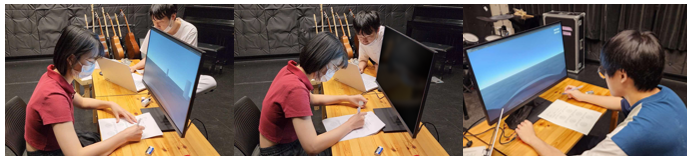
\includegraphics[width=0.8\textwidth]{A_thesis/figures/036.png}
\caption{Three experimental conditions}
\end{figure}

Under Only-visual conditions, participants do not use the MotionPerformer and rely on visual cues to judge and describe the current movement status of the vehicle. Under Only-haptic conditions, participants hold the device and depend entirely on the haptic feedback provided by MotionPerformer to describe the vehicle's current movement state. For Visual-haptic conditions, participants hold the MotionPerformer while watching the monitor, using both visual and haptic to judge the vehicle's movement state.

The motion tests will encompass various movements including fast forward, slow forward, fast backward, slow backward, fast left, slow left, fast right, and slow right. To circumvent participants' inherent directional biases, the sequence of tests will be randomized. The final sequence is slow left turn, fast left turn, fast forward, slow backward, fast backward, slow right turn, slow forward, and fast right turn. After each test, the vehicle returns to its initial state, ensuring that the next test does not build upon the prior one's movement state. Each test involves a single type of motion, such as a left turn or a forward movement, and compound movements are not included in the tests. Unless otherwise required, each test is conducted only once.

The motion detection method draws inspiration from \cite{paper36}, using drawing as a mode of testing. Staff input commands via keyboard, and participants, upon feeling the device's operations, will depict each motion's status graphically. The central black area in the figure signifies the position of the virtual vehicle/avatar, and each chart should indicate both the direction of displacement (forward or backward) or rotation angle (left or right) and the perceived speed, represented by the thickness of the pen line.

\subsection{Experiment Preparations}
Before the experiment, participants will be introduced to the fundamental information about the device and system and its operation, followed by a swift test to ascertain their preferred mode of operation. As documented in \cite{ref_motion001}, participants exhibit two primary patterns of perceiving movement direction: the device's motion either aligns or contrasts with the actual direction of movement, with both preferences appearing with equal probability. Consequently, it's crucial to explain the correlation between the device's movement data and the physical object's movement data to the participants before starting the formal testing.

Also, from earlier pilot tests, we learned that the device might pinch the user's hand, potentially affecting their assessment. Therefore, participants are advised to adjust their grip to a comfortable state where they can perceive the mechanical feedback but not impede the device's normal functioning. Each test will be performed once per session, barring any special requirements.

\subsection{Experiment Procedure}
Upon completion of preparations, participants will conduct three rounds of testing, including "Only-visual", "Only-haptic" and "Visual-haptic". Each round of testing consists of eight sub-tests, followed by filling out the questionnaire.
\begin{figure}[h]
\centering
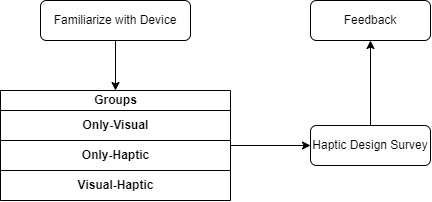
\includegraphics[width=0.7\textwidth]{A_thesis/figures/037.png}
\caption{Flowchart of Experiment 1}
\end{figure}

At the end of Experiment 1, participants will be asked to indicate on the subsequent graphic the haptic sensations they experienced in their palms. These inputs will serve as valuable recommendations for future design modifications and feedback on the overall device performance and user experience.

\begin{figure}[h]
\centering
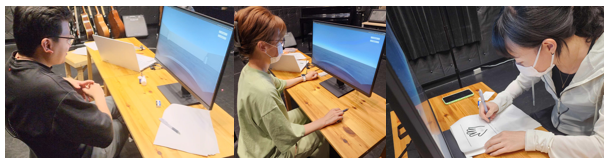
\includegraphics[width=0.8\textwidth]{A_thesis/figures/038.png}
\caption{Photos during Experiment 1}
\end{figure}

\textbf{For further details on the experimental questionnaire, please refer to the appendix 'C'.}

\subsection{Results}
\subsubsection{Motion Information Diagram}
\begin{figure}[h]
\centering
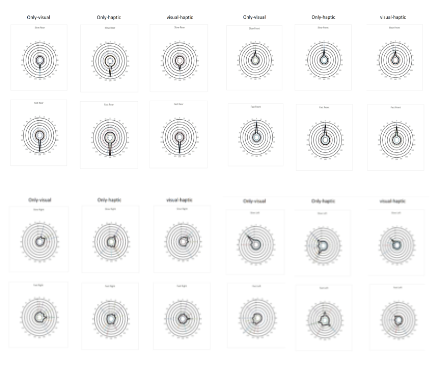
\includegraphics[width=0.5\textwidth]{A_thesis/figures/039.png}
\caption{Results of motion information diagram}
\end{figure}

\textbf{Please refer to the appendix 'E'.}


\subsubsection{Haptic Sensation of Hand}

\begin{figure}[h]
\centering

\includegraphics[width=0.3\textwidth]{A_thesis/figures/016.png}
\caption{Results of the hand diagram}
\end{figure}



\subsubsection{Feedback Recording}
001: "I think having haptic feedback in games or while driving would be quite magical. However, the feeling of moving forward and backward is more intense than turning."

002: "Haptic can provide me the intensity of movement which is something that only-visual cannot provide. But only-haptic cannot precisely provide me the information of the distance moved. So, the combination of haptic and visual can provide the best experience."

003: "My hand got a bit pinched."

004: "Everything felt faster and farther when haptic was involved, especially in the mixed condition while the visual didn’t feel that fast/far, the haptic felt very fast and far."

005: "After using the device, the physical reference became easier to grasp, and the experience became more intense."

006: "Haptic touch gave me a stronger feeling when the car moves than visual."

007: "Visual haptic is much better for the experience. The haptic device is good for sensing speed."

008: ”The feeling from haptic is strong, I can easily tell direction and angle, but not so much for speed changing. Haptic on palm is good, can keep fingers free for other things. When seeing and feeling at same time, I look at vision first but haptic feels faster.”

009: “Speed of vision and haptic not same, in experiment design, setting reference for haptic and vision speed first can help a lot in understanding later experiments.”

010: "When using only visual, it's difficult to perceive the angle. Only-haptic needs time to respond to left and right judgements."


\section{Experiment 2: User Experience Test}
\subsection{Experiment Description}
The purpose of Experiment 2 is to evaluate the integrated user experience of using the MotionPerformer in simulated scenarios. This experiment is divided into two rounds of testing according to usage scenarios: the first round involves passive scenario testing, and the second round involves active scenario testing.

In the passive scenario, we employ the Wizard-of-Oz method\cite{paper37}, where staff will simulate the operation of the vehicle's motion in a virtual space by an AI system in the driving system. Users are required only to receive the vehicle's motion information through a display or the MotionPerformer.

In the active scenario, users themselves are required to control the vehicle's movement, while simultaneously receiving the vehicle's motion information via a display or the MotionPerformer.

Moreover, within each round of testing, we adopt the within/without method. This approach facilitates the comparative testing of user's overall experience of the MotionPerformer when receiving both visual and haptic motion information via a display and the MotionPerformer, against scenarios when they are only receiving visual motion information through a display without using the MotionPerformer. 
And to avoid bias, odd-numbered participants will undertake the 'within' test first, followed by the 'without' test. Conversely, even-numbered participants will undertake the 'without' test and proceeding to the 'within' test.

Upon the conclusion of each experiment, they will be requested to fill out a relevant survey questionnaire.The questionnaire for this experiment is composed of two parts. The first eight options stem from the experiment and survey on the sense of agency \cite{paper38} . The final eight options are informed by a user experience survey within a gaming context\cite{paper39}.

\subsection{Experiment Procedure}

\begin{figure}[h]
\centering
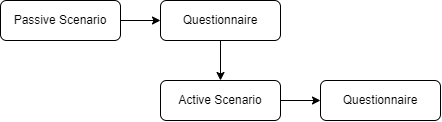
\includegraphics[width=0.8\textwidth]{A_thesis/figures/042.png}
\caption{Flowchart of Experiment 2}
\end{figure}

Upon completion of Experiment 1, and after briefly introducing the procedure of Experiment 2 to the participants, Experiment 2 will commence directly. Participants will first undertake the initial round of testing in passive usage scenarios simulating AI driving. The virtual vehicle will operate automatically, requiring no active manipulation by the participants, who will experience the motion state of the virtual vehicle through the screen and the MotionPerformer. This includes two sub-tests under both 'within' and 'without' conditions. Each sub-test will last for one minute, followed by a requirement for participants to complete the questionnaire.

After the conclusion of the two sub-tests in the first round, the second round of active usage scenario test will begin. In this phase, participants will actively control the motion of the vehicle using the arrow keys on the keyboard while experiencing the motion state of the virtual vehicle through the screen and MotionPerformer. This round also includes 'within' and 'without' tests, each lasting for one minute, followed by the completion of the questionnaire.

\textbf{For further details on the experimental questionnaire, please refer to the appendix 'D'.}

\begin{figure}[h]
\centering
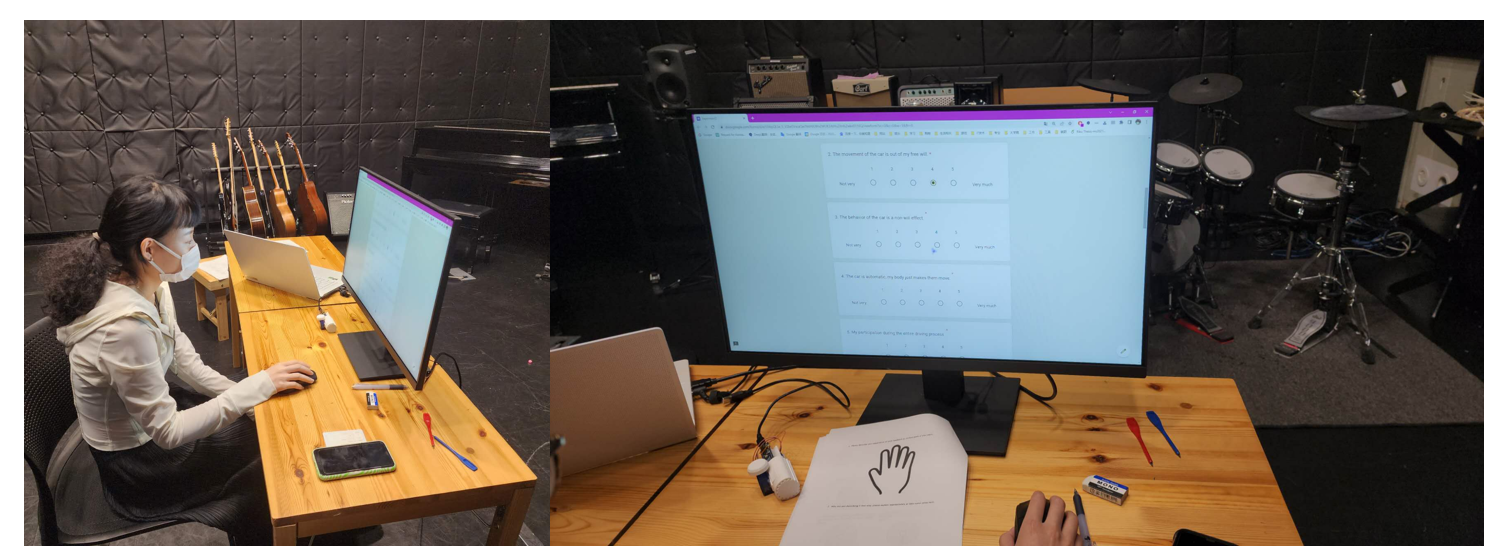
\includegraphics[width=0.8\textwidth]{A_thesis/figures/018.png}
\caption{Photos of the experiment2}
\end{figure}

\subsection{Results}
\begin{figure}[h]
\centering
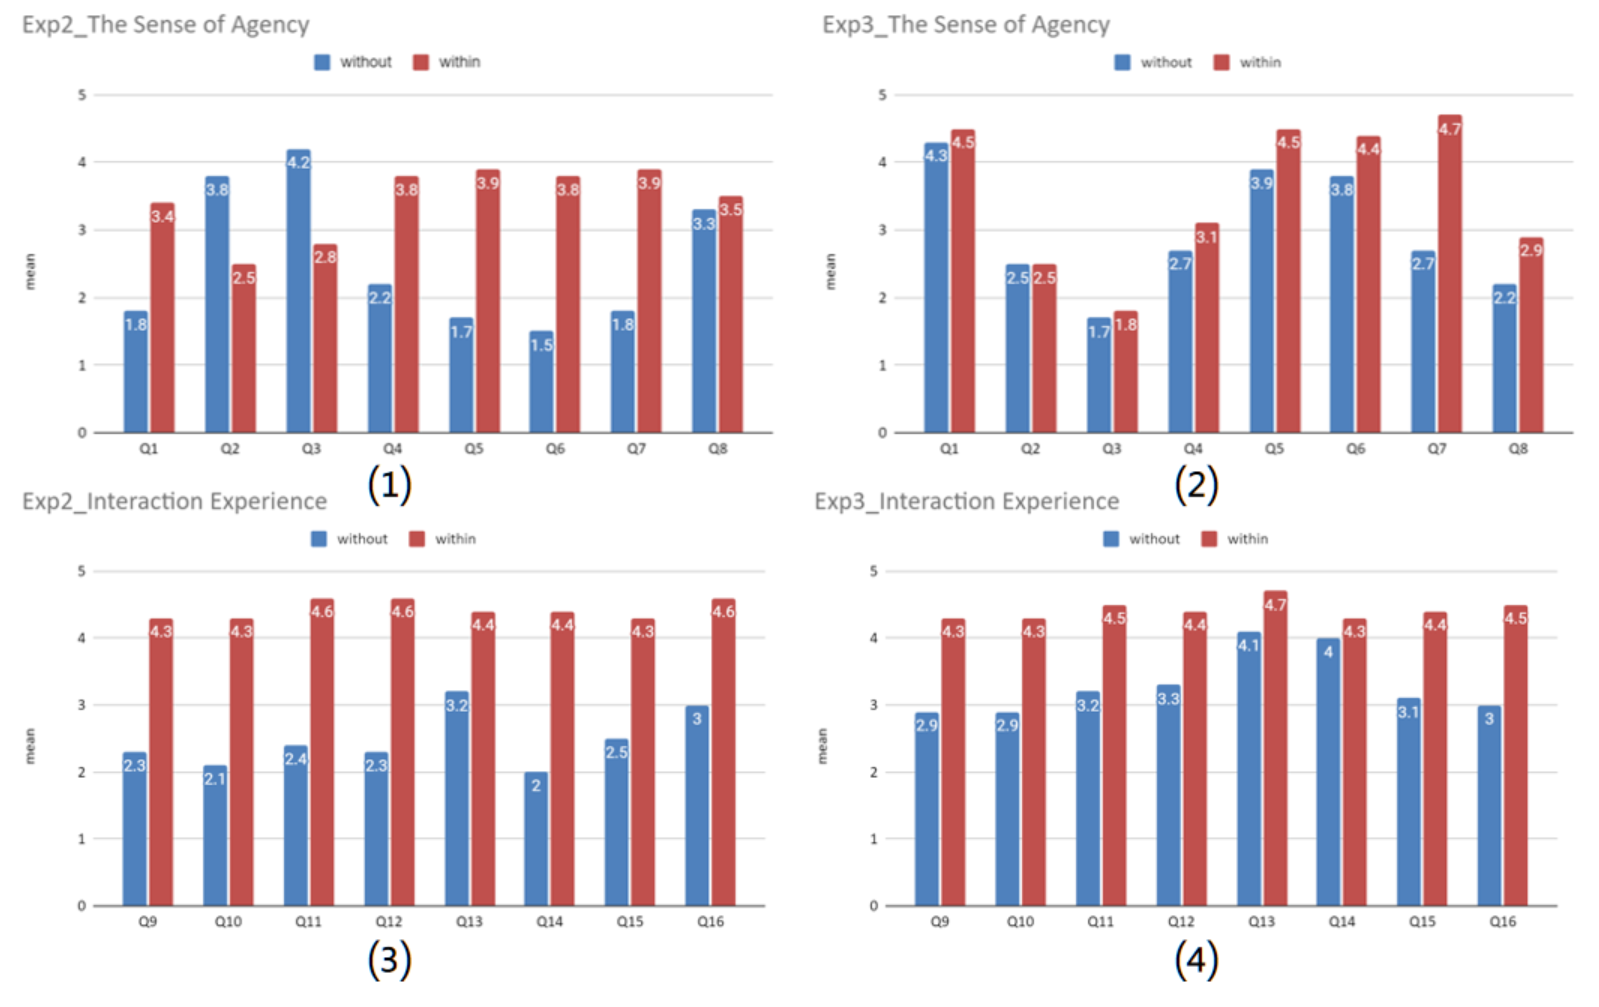
\includegraphics[width=0.8\textwidth]{A_thesis/figures/043.png}
\caption{Data visualization of experiment 2 results}
\end{figure}

After collecting all the data, we visualized in the form of bar graphs. According to the direction of the questionnaire and the different usage scenarios, the data is presented in four different charts, as seen in Figure 4.8: (1) the sense of agency in passive scenarios, (2) the sense of agency in active scenarios, (3) the sense of interaction in passive scenarios, and (4) the sense of interaction in active scenarios. Within these charts, the 'with' and 'without' experiment conditions are differentiated using blue and red respectively. Blue represents the experiment results without using the MotionPerformer, and red represents the experiment results with the use of the MotionPerformer.

On the whole, it can be roughly observed that the use of the MotionPerformer enhances the user's sense of agency and interaction in driving, with some elements even showing a quite significant improvement. A more detailed and specific analysis of the experiment results will be presented in the next chapter.

\textbf{For more data sources data, please refer to the appendix 'F'.}



